\documentclass{beamer}
\usetheme{Warsaw}
\usepackage{nhtvslides}
\usepackage{graphicx}
\usepackage{listings}
\lstset{language=CAML,
basicstyle=\ttfamily\footnotesize,
frame=shadowbox,
breaklines=true}
\usepackage[utf8]{inputenc}

\title{Building a physics engine - part 4: broad phase of collision detection}

\author{Dr. Giuseppe Maggiore}

\institute{NHTV University of Applied Sciences \\ 
Breda, Netherlands}

\date{}

\begin{document}
\maketitle

\begin{frame}{Table of contents}
\tableofcontents
\end{frame}

\section{Broad phase of collision detection}
\begin{slide}{Broad phase of collision detection}{Increasing performance, in general}{
\item What is the fastest instruction?
\pause
\item The one that is not run!
}\end{slide}

\begin{slide}{Broad phase of collision detection}{Increasing performance, in collision detection}{
\item How do we increase performance in a collision detection system?
\item Quickly and cheaply exclude pairs of colliders
\item Process known as \textit{collision culling}
\begin{itemize}
\item We \textit{ensure lack} of collisions
\item \textit{Presence is ensured} only during narrow phase
\end{itemize}
\item Akin to frustum/occlusion culling
}\end{slide}

\section{Bounding spheres}
\begin{slide}{Collision culling}{Bounding spheres}{
\item An obvious choice is bounding spheres
\item Identical w.r.t. rotation
\item Fast to check against other spheres
}\end{slide}

\begin{slide}{Collision culling}{Intersection of bounding spheres}{
\item Two spheres, $\langle C_0, r_0 \rangle$ and $\langle C_1, r_1 \rangle$
\item Intersection when $|C_1 - C_0| \leq r_1 + r_0$
\item Intersection also when $|C_1 - C_0|^2 \leq (r_1 + r_0)^2$
}\end{slide}

\begin{slide}{Collision culling}{Intersection of bounding spheres}{
\item If the spheres are moving, then we can increase their radii by their speed
\item Or we can project their relative speed
\pause
\item $\sigma = |(V_1 - V_2) \cdot \frac{C_1 - C_0}{|C_1 - C_0|}|$
\item $|C_1 - C_0| \leq r_1 + r_0 + \sigma$
}\end{slide}

\begin{frame}{Moving spheres}
\center
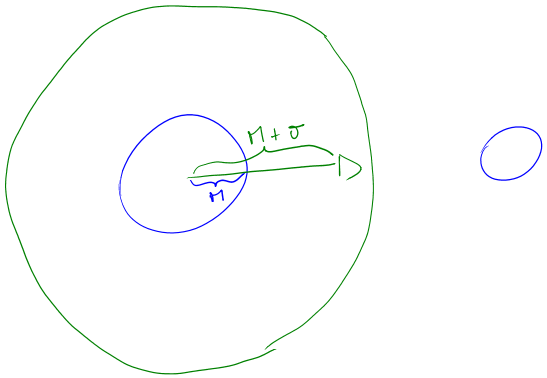
\includegraphics[height=5cm]{Pics/MovingSpheres.png}
\end{frame}

\section{Space partitioning}
\begin{slide}{Space partitioning}{Space partitioning}{
\item We can also decompose space in axis-aligned-bounding-boxes (``bins'')
\item Even earlier no-collision determination
\item This would reduce the number of sphere-to-sphere checks
}\end{slide}

\begin{frame}{SLIDE}
\center
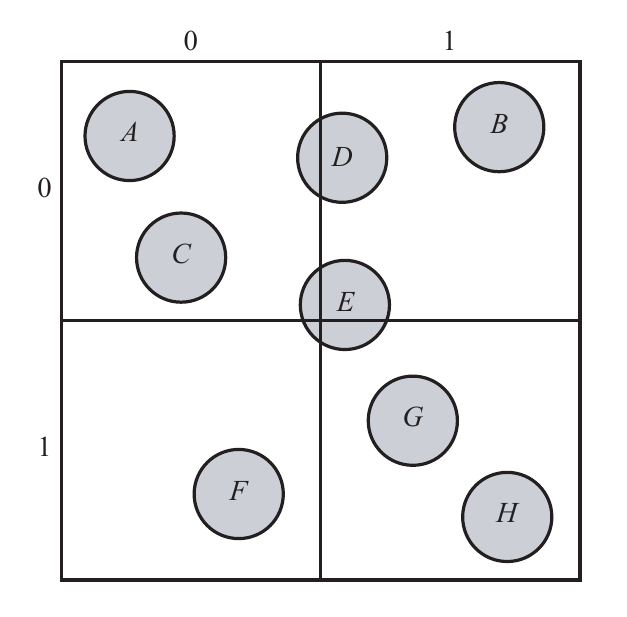
\includegraphics[height=5cm]{Pics/SpacePartitioning.png}
\end{frame}

\begin{slide}{Space partitioning}{Space partitioning}{
\item We can divide space in \textit{bins}; each bin is an AABB
\item Sphere intersection with an AABB bounded by points $L$ and $U$ 
\item No intersection if $|C_j - L_j| \leq r_j + \sigma_j$ or $C_j - U_j| \leq r_j + \sigma_j$ for all axes $j = x,y,z$
}\end{slide}

\begin{slide}{Space partitioning}{Space partitioning}{
\item When a sphere moves, it only moves to a neighbouring bin; less checks
\item We can find the right bin directly with modulus operations (hashing)
}\end{slide}

\section{Bounding boxes}
\begin{slide}{Axis aligned bounding boxes}{AABB intersection}{
\item A simple and powerful algorithm exists for determining intersection groups of AABBs
\item It is particularly fast, especially if the AABBs do not move too much between frames
}\end{slide}

\begin{slide}{Axis aligned bounding boxes}{AABB intersection}{
\item Update AABBs (if needed)
\item Insertion sort the extremes of each box; one list for every axis (2 for 2D, 3 for 3D, etc.)
\begin{itemize}
\item After the first frame the list is \textit{nearly sorted}
\item $O(n)$ complexity
\end{itemize}
}\end{slide}

\begin{slide}{Axis aligned bounding boxes}{AABB intersection}{
\item Run sweep algorithm
\begin{itemize}
\item Active intervals $= \emptyset$
\item When a beginning value is encountered, add it as intersecting all active intervals; add it to active intervals
\item When end value is encountered, remove it from the active intervals
\end{itemize}
\item Intersections must be confirmed across all axes
}\end{slide}

\begin{slide}{Oriented bounding boxes}{OBB}{
\item An OBB is characterized by a center and three directions (columns of the rotation matrix)
\item The vertices are $P = C + \sigma_0 e_0 U_0 + \sigma_1 e_1 U_1 + \sigma_2 e_2 U_2$
\begin{itemize}
\item $\sigma_i = 1$ or $\sigma_i = -1$
\item $e_i$ are the half extents
\end{itemize}
}\end{slide}

\begin{slide}{Oriented bounding boxes}{OBB SAT}{
\item With the separating axis test, it may seem that we need to test $6$ face normals for one, $6$ for the other, and $12^2 = 144$ edge pair cross products
\item That's quite a lot!
}\end{slide}

\begin{slide}{Oriented bounding boxes}{OBB SAT}{
\item The OBB is symmetric, so many tests are redundant
\begin{itemize}
\item Three unique face directions
\item Three unique edge directions
\end{itemize}
\item The minimum number of required tests is $3$ face normals for one, $3$ for the other, and $3^2 = 9$ edge pair cross products
}\end{slide}

\begin{slide}{Oriented bounding boxes}{OBB SAT}{
\item We project both OBBs onto one of the unique potential separating directions $Q + tD$
\item We look for an extremal vertex such that $\max_P D \cdot (P - Q)$
\item $D \cdot (P - Q) = D \cdot (C + \sigma_0 e_0 U_0 + \sigma_1 e_1 U_1 + \sigma_2 e_2 U_2 - Q)$
}\end{slide}

\begin{slide}{Oriented bounding boxes}{OBB SAT}{
\item We are maximizing, so we do not try all the $\sigma_i$ combinations
\begin{eqnarray}
D \cdot (P - Q) &=& D \cdot (C + \sigma_0 e_0 U_0 + \dots  - Q) \\
&=& D \cdot (C - Q) + \sigma_0 e_0 D \cdot U_0 + \dots \\
&=& D \cdot (C - Q) + \sum_{i=0}^2 |e_i D \cdot U_i|
\end{eqnarray}
}\end{slide}

\begin{slide}{Oriented bounding boxes}{OBB SAT}{
\item Maximization results in $\max_P D \cdot (P - Q) = \underbrace{D \cdot (C - Q)}_{\gamma} + \underbrace{\sum_{i=0}^2 |e_i D \cdot U_i|}_{r}$
\item Minimization results in $\min_P D \cdot (P - Q) = D \cdot (C - Q) - \sum_{i=0}^2 |e_i D \cdot U_i|$
\item The interval is thus $[\gamma - r, \gamma + r]$
\item \textbf{Important:} the separating directions \textit{must be unit length}, and the edges as well
}\end{slide}

\begin{slide}{Oriented bounding boxes}{OBB SAT}{
\item We project both OBBs onto their intervals $[\gamma_1 - r_1, \gamma_1 + r_1]$ and $[\gamma_2 - r_2, \gamma_2 + r_2]$
\item They intersect when $|\gamma_2 - \gamma_1| < r_1 + r_2$
}\end{slide}

\begin{slide}{Oriented bounding boxes}{OBB SAT - final optimization}{
\item Some separating directions are taken from the cross product of two edge directions: $D = U_i^1 \times U_k^2$
\item When we plug those directions $D$ in the above formulas, we get $U_i^1 \times U_k^2 \cdot U_j^1$
\item We can rewrite $U_i^1 \times U_k^2 \cdot U_j^1 = U_i^1 \times U_j^1 \cdot U_k^2$
\item We can cache the products $U_i^1 \times U_j^1$, so we do not have to recompute them
}\end{slide}

\begin{slide}{Moving objects}{Moving objects}{
\item We ignore the angular velocity; does not improve much, and is very complex to handle
\item We can enlarge the interval radii by projecting the current relative velocity onto the separating direction
\item $s = D \cdot (V_2 - V_1)$
}\end{slide}

\section{Further optimizations}
\begin{slide}{Further optimizations}{Islands}{
\item Apply collision response system only to groups of objects in contact
\item Flood-fill algorithm
}\end{slide}

\begin{slide}{Further optimizations}{Sparse matrices for collision response}{
\item Avoid multiplying lots of zeroes
\item Store matrix row as list of \texttt{int * float} entries
}\end{slide}

\section{Assignment}
\begin{slide}{Assignment}{Assignment}{
\item Before the end of next week
\item Group-work archive/video on Natschool or uploaded somewhere else and linked in your report
\item Individual report by each of you on Natschool
\item Build a broad phase collision detector that supports a combination of bounding spheres, AABBs, bins, and OBBs
}\end{slide}

\begin{frame}{That's it}
\center
\fontsize{18pt}{7.2}\selectfont
Thank you!
\end{frame}

\end{document}


\begin{slide}{SECTION}{SLIDE}{
\item i
}\end{slide}

\begin{frame}[fragile]{SLIDE}
\begin{lstlisting}
CODE
\end{lstlisting}
\end{frame}

\begin{frame}{SLIDE}
\center
%\includegraphics[height=5cm]{Pics/recursive_multiplier.png}
\end{frame}
